\begin{myprops}
	\begin{itemize}
		\iftoggle{eleve}{%
			\item Le symétrique d'une droite par rapport à\hrulefill
			
			\vspace*{0.2cm}
			\hrulefill			
			
			\item Si deux droites sont \hrulefill
			
			\vspace*{0.2cm}
			\hrulefill			
		}{%
			\item Le symétrique d'une droite par rapport à une droite ou un point est \kw{une autre droite}.
			\item Si deux droites sont symétriques \kw{par rapport à un point} alors elles sont \kw{parallèles}.
		}		
	\end{itemize}
\end{myprops}

\begin{myexs}
	\begin{multicols}{2}
		\begin{center}
			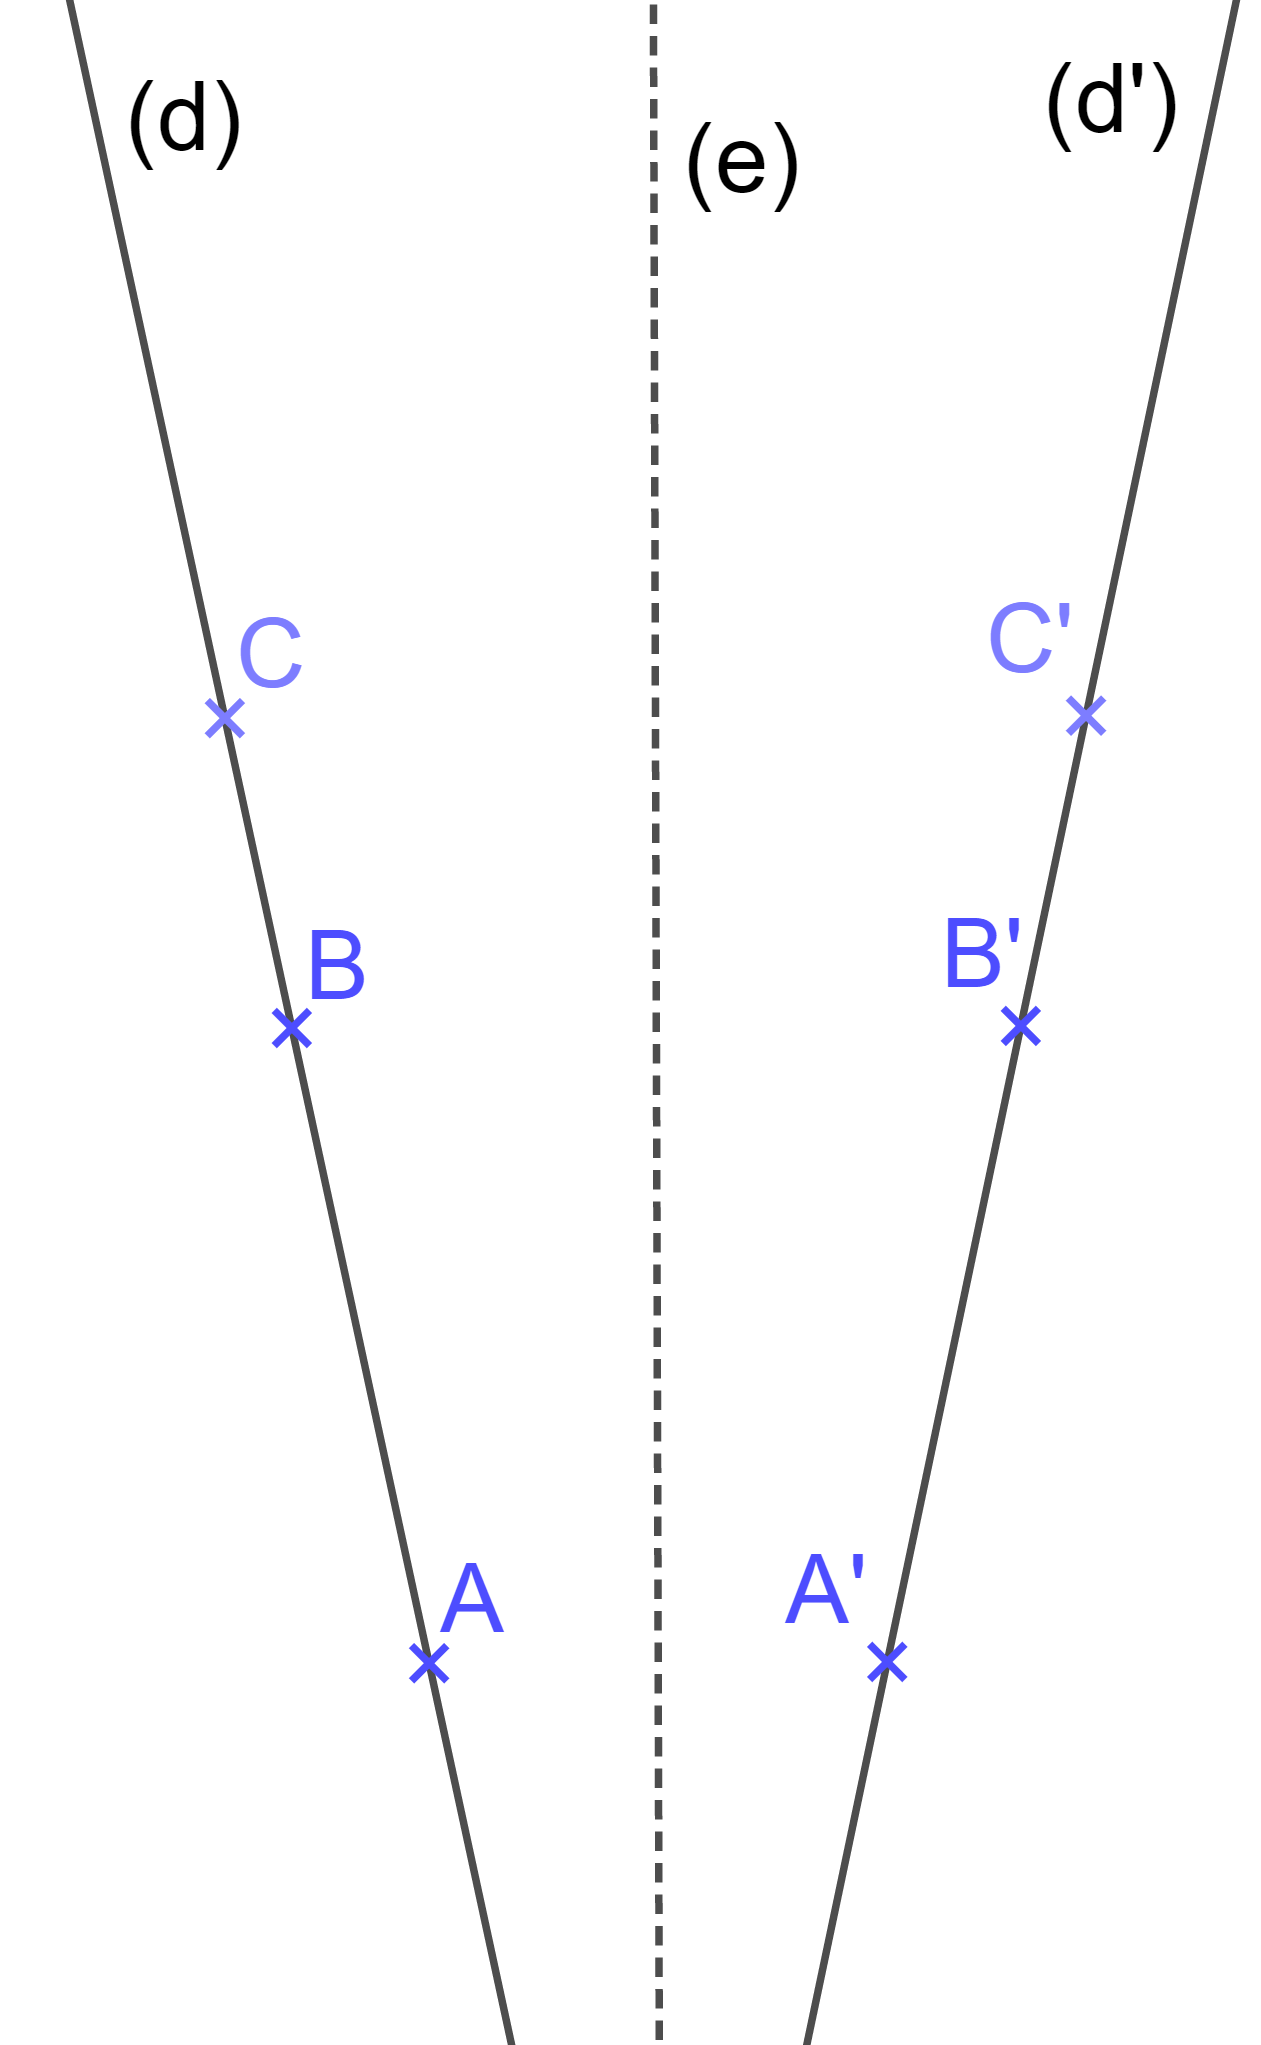
\includegraphics[scale=0.2]{sym_droites1}
		\end{center}

		\begin{itemize}
			\iftoggle{eleve}{%
				\item Les points $A$, $B$ et $C$ sont alignés,
				
				\vspace*{0.2cm}
				 donc\hrulefill
				
				\vspace*{0.2cm}
				\hrulefill
				
				\vspace*{0.2cm}
				\hrulefill
			}{%
				\item Les points $A$, $B$ et $C$ sont alignés, donc $A'$, $B'$ et $C'$ leur symétriques par rapport à la droite $(e)$ sont aussi alignés.
			}
			
		\end{itemize}	
		
		\begin{center}
			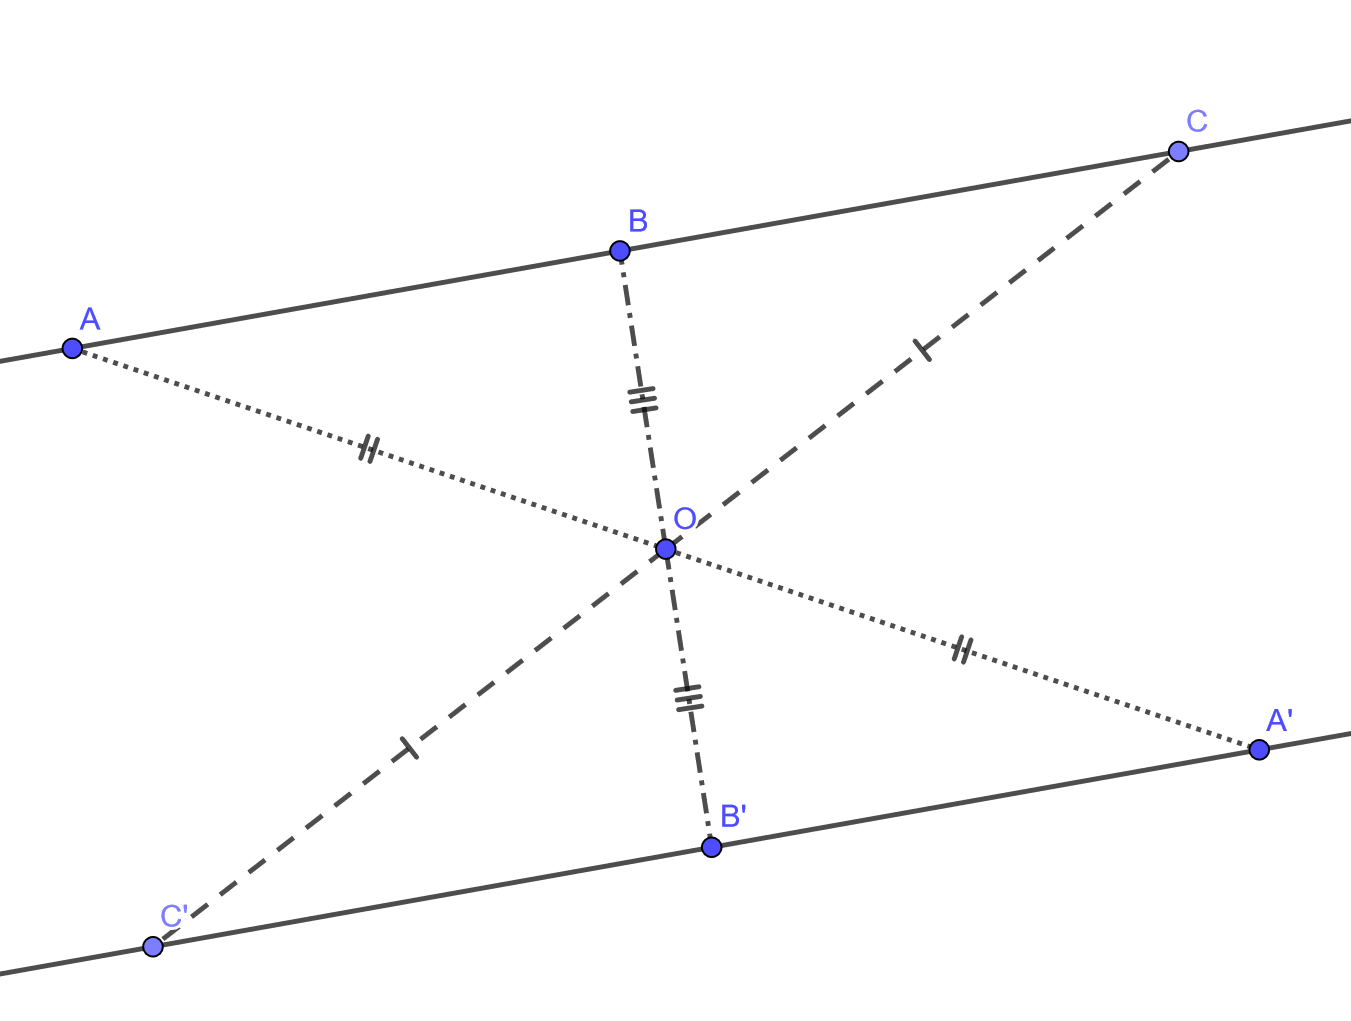
\includegraphics[scale=0.2]{sym_droites2}
		\end{center}
	
		\begin{itemize}
			\iftoggle{eleve}{%
				\item Les points $A$, $B$ et $C$ sont alignés,
				
				\vspace*{0.2cm}
				donc\hrulefill
				
				\vspace*{0.2cm}
				\hrulefill
				
				\vspace*{0.2cm}
				\hrulefill
				
				
				\item La droite $(AB)$ est \hrulefill 
				
				\vspace*{0.2cm}
				\hrulefill.
			}{%
				\item Les points $A$, $B$ et $C$ sont alignés, donc $A'$, $B'$ et $C'$ leur symétriques par rapport au point $O$ sont alignés.
				\item La droite $(AB)$ est parallèle à la droite $(A'B')$.
			}
			
		\end{itemize}
	\end{multicols}
\end{myexs}

\begin{myprop}
	\iftoggle{eleve}{%
		Le symétrique d'un segment par rapport \hrulefill 
		
		\vspace*{0.2cm}
		
		\hrulefill
		
		\vspace*{0.2cm}
		
		\hrulefill
	}{%
	Le symétrique d'un segment par rapport à une droite ou un point est un segment \kw{de même longueur}.
	}
\end{myprop}

\begin{myex}
	\begin{center}
		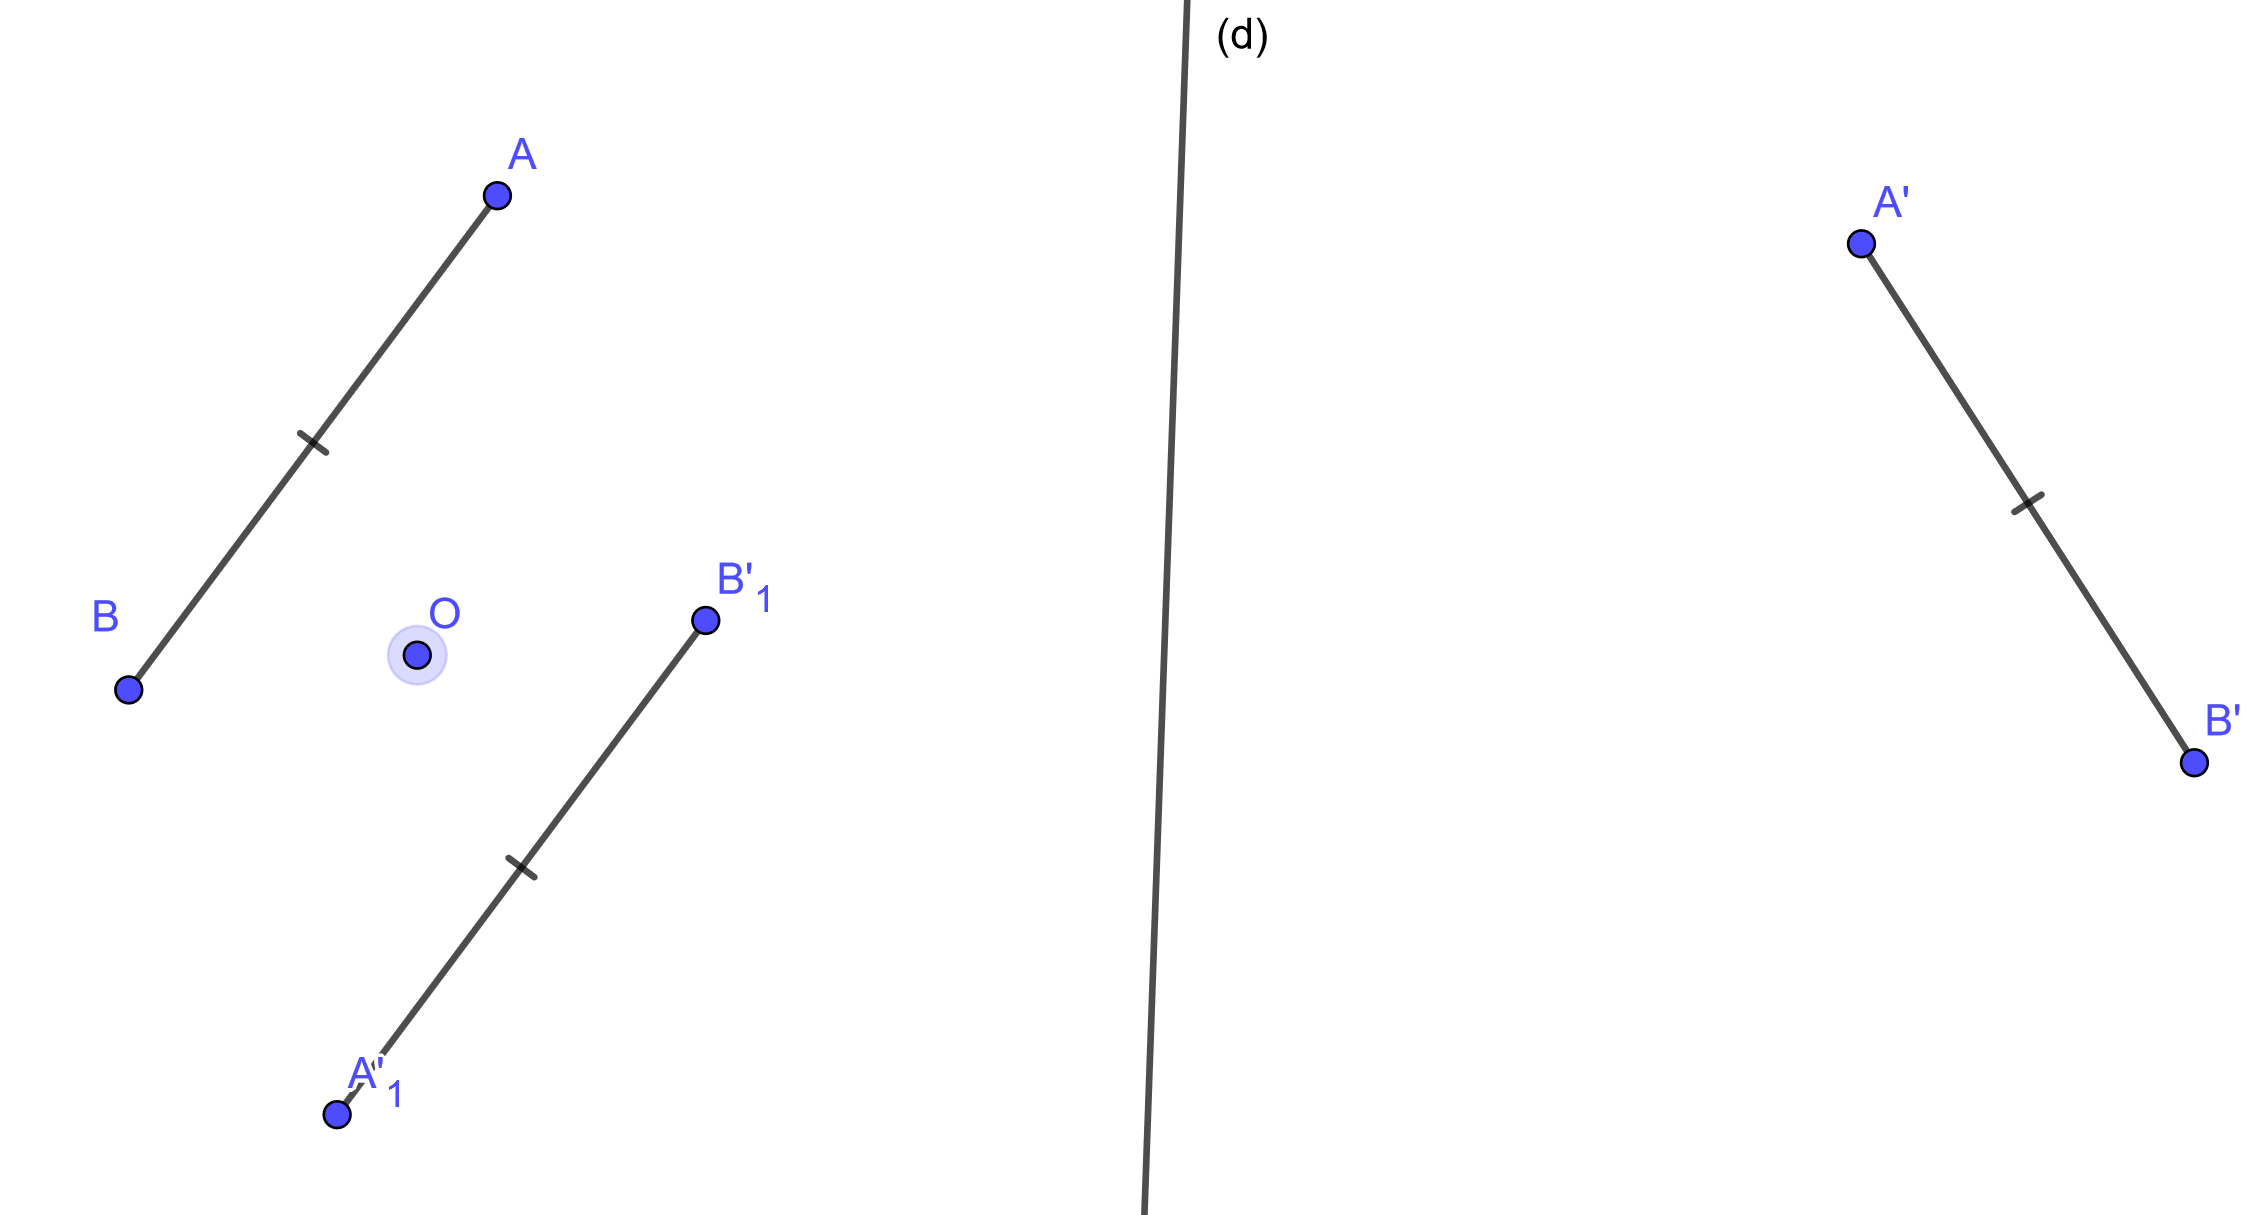
\includegraphics[scale=0.15]{sym_seg}
	\end{center}

\iftoggle{eleve}{%
	Le segment $[A'B']$ est le symétrique du segment $[AB]$ par rapport à \hrulefill
	
	\vspace*{0.2cm}
	
	\hrulefill
	
	\vspace*{0.2cm}
	
	\hrulefill
}{%
Le segment $[A'B']$ est le symétrique du segment $[AB]$ par rapport à la droite $(d)$ et $[A'_1B'_1]$ est le symétrique de $[AB]$ par rapport au point $O$. 
On a $AB$ = $A'B'$ = $A'_1B'_1$.
}
	
\end{myex}

\begin{myprop}
	\begin{itemize}
		\iftoggle{eleve}{%
			\item Le symétrique d'une figure par rapport à \hrulefill 
			
			\vspace*{0.2cm}
			
			\hrulefill
			\item La symétrie conserve : \hrulefill 
			
			\vspace*{0.2cm}
			
			\hrulefill
		}{%
			\item Le symétrique d'une figure par rapport à une droite ou un point est une figure \kw{de même forme}.
			\item La symétrie conserve : \kw{les longueurs, l'alignement, les mesures d'angles et les aires}.			
		}
		
	\end{itemize}
	
\end{myprop}

\begin{myex}
	\begin{center}
		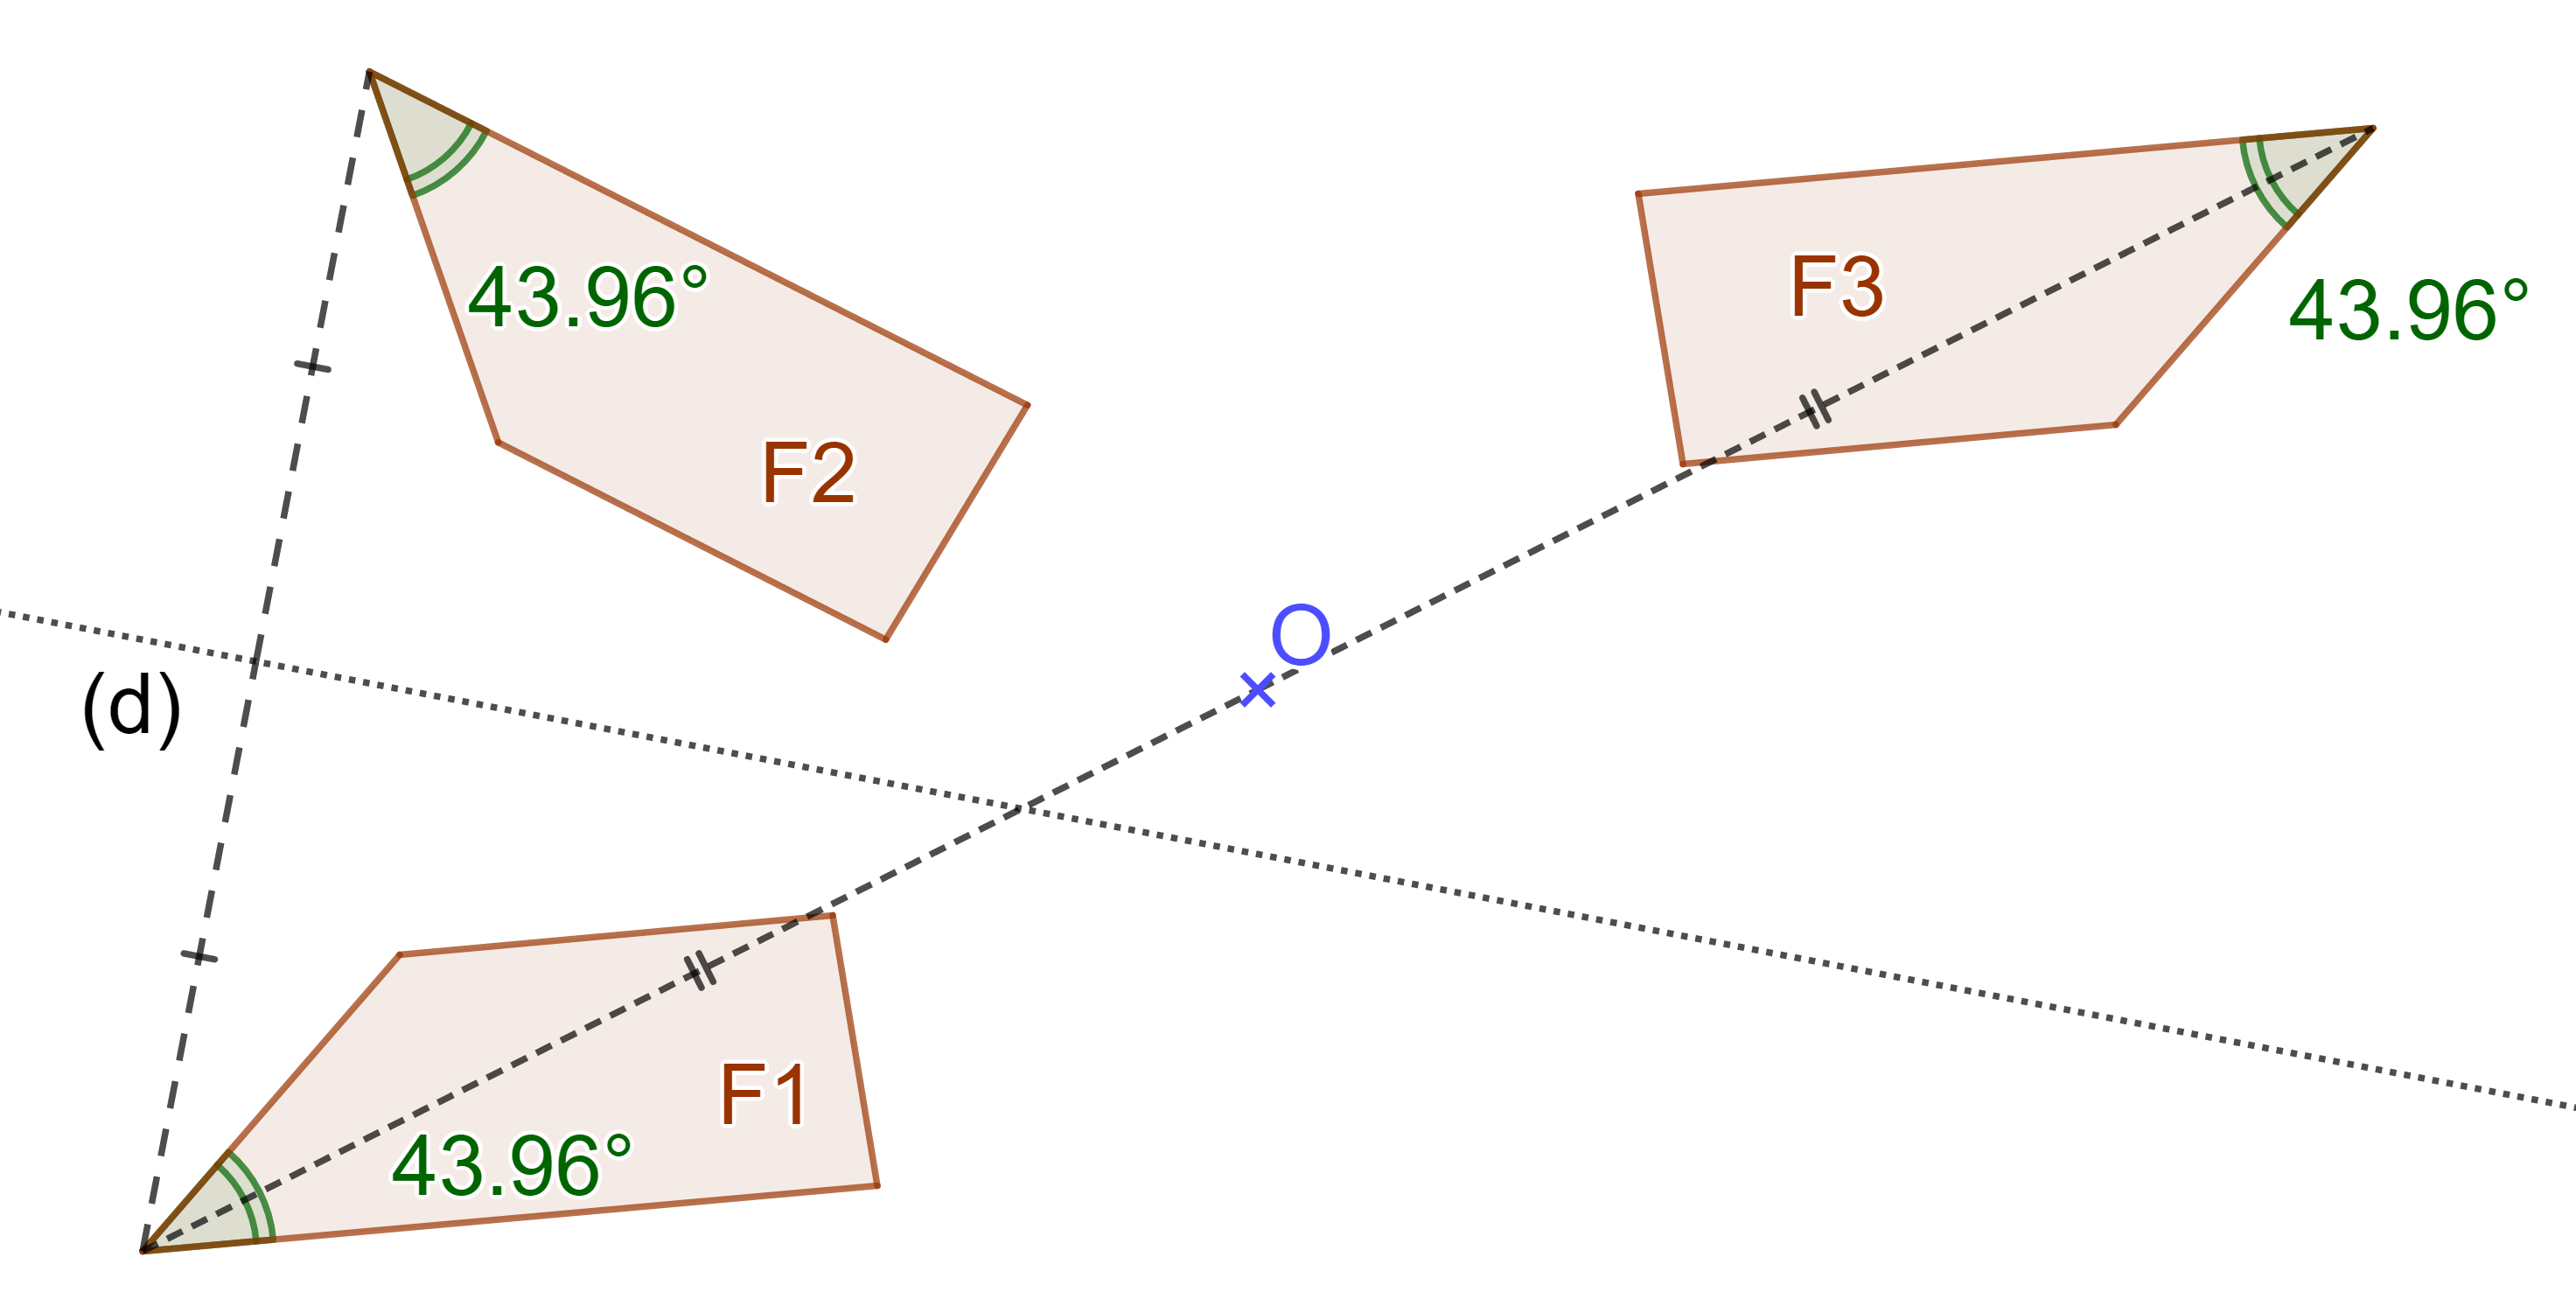
\includegraphics[scale=0.18]{sym_figures}
	\end{center}
	
	\iftoggle{eleve}{%
		$F2$ et $F3$ sont les symétriques de $F1$ respectivement par rapport à \hrulefill 
		
		\vspace*{0.2cm}
		
		\hrulefill	
	}{%
		$F2$ et $F3$ sont les symétriques de $F1$ respectivement par rapport à la droite $(d)$ et au point O. Elles ont les mêmes angles, le même périmètre et la même aire.
	}
\end{myex}

